%% ─────────────────────────────────────────────────────────────────────────────
%% ZEPHYR — PROJECT SPECIFICATION DOCUMENT
%% Boxing Coach Management System
%% Compiler: pdfLaTeX | Version: 2.0 | 2026
%% ─────────────────────────────────────────────────────────────────────────────

\documentclass[11pt,a4paper]{article}

%% ── PACKAGES ─────────────────────────────────────────────────────────────────
\usepackage[a4paper, top=2cm, bottom=2cm, left=2.2cm, right=2.2cm]{geometry}
\usepackage[T1]{fontenc}
\usepackage[utf8]{inputenc}
\usepackage{lmodern}
\usepackage{microtype}
\usepackage{xcolor}
\usepackage{booktabs}
\usepackage{tabularx}
\usepackage{longtable}
\usepackage{array}
\usepackage{colortbl}
\usepackage{multirow}
\usepackage{graphicx}
\usepackage{enumitem}
\usepackage{titlesec}
\usepackage{fancyhdr}
\usepackage{tocloft}
\usepackage{hyperref}
\usepackage{parskip}
\usepackage{mdframed}
\usepackage{tikz}
\usepackage{fontawesome5}
\usepackage{setspace}
\usepackage{caption}
\usepackage{float}
\usepackage{pgfgantt}
\usepackage{adjustbox}

%% ── COLORS ───────────────────────────────────────────────────────────────────
\definecolor{Black}{HTML}{1A1A1A}
\definecolor{DarkGray}{HTML}{3D3D3D}
\definecolor{MidGray}{HTML}{666666}
\definecolor{LightGray}{HTML}{ECECEC}
\definecolor{BorderGray}{HTML}{CCCCCC}
\definecolor{OffWhite}{HTML}{F8F8F8}
\definecolor{White}{HTML}{FFFFFF}

\definecolor{RedMain}{HTML}{C62828}
\definecolor{RedDark}{HTML}{8E0000}
\definecolor{RedLight}{HTML}{FFEBEE}

\definecolor{Green}{HTML}{2E7D32}
\definecolor{Orange}{HTML}{EF6C00}

%% ── HYPERREF ─────────────────────────────────────────────────────────────────
\hypersetup{
  colorlinks=true,
  linkcolor=RedMain,
  urlcolor=RedDark,
  pdftitle={Zephyr — Project Specification},
  pdfauthor={Zephyr Dev Team},
}

%% ── BASIC TYPOGRAPHY ─────────────────────────────────────────────────────────
\setlength{\parskip}{4pt plus 1pt minus 1pt}
\setlength{\parindent}{0pt}
\onehalfspacing

%% ── SECTION STYLING ──────────────────────────────────────────────────────────
\titleformat{\section}
  {\color{Black}\Large\bfseries}
  {}
  {0pt}
  {\makebox[0pt][l]{\rule[-2pt]{0.8cm}{2.4pt}}\quad\thesection\hspace{0.5em}#1}
  []

\titleformat{\subsection}
  {\color{Black}\large\bfseries}
  {\thesubsection}
  {0.5em}
  {#1}

\titleformat{\subsubsection}
  {\color{DarkGray}\normalsize\bfseries}
  {\thesubsubsection}
  {0.5em}
  {#1}

\titlespacing*{\section}{0pt}{14pt}{8pt}
\titlespacing*{\subsection}{0pt}{10pt}{4pt}
\titlespacing*{\subsubsection}{0pt}{8pt}{2pt}

%% ── HEADER / FOOTER ──────────────────────────────────────────────────────────
\setlength{\headheight}{14pt}
\pagestyle{fancy}
\fancyhf{}
\fancyhead[L]{\small\color{MidGray}Zephyr v2.0 — Project Specification}
\fancyhead[R]{\small\color{MidGray}Confidential}
\fancyfoot[C]{\small\color{MidGray}— \thepage\ —}
\renewcommand{\headrulewidth}{0.5pt}
\renewcommand{\footrulewidth}{0pt}
\renewcommand{\headrule}{\color{Black}\hrule height 0.5pt}

%% ── TABLE HELPERS ────────────────────────────────────────────────────────────
\newcolumntype{L}[1]{>{\raggedright\arraybackslash}p{#1}}
\newcolumntype{C}[1]{>{\centering\arraybackslash}p{#1}}
\newcolumntype{R}[1]{>{\raggedleft\arraybackslash}p{#1}}

\newcommand{\hrow}{\rowcolor{Black}\color{White}\bfseries}
\newcommand{\altrow}{\rowcolor{OffWhite}}

%% ── SIMPLE LABELS ────────────────────────────────────────────────────────────
\newcommand{\methodget}{\texttt{GET}}
\newcommand{\methodpost}{\texttt{POST}}
\newcommand{\methodput}{\texttt{PUT}}
\newcommand{\methoddelete}{\texttt{DELETE}}
\newcommand{\roleadmin}{[Admin]}
\newcommand{\rolecoach}{[Coach]}

\newmdenv[
  backgroundcolor=OffWhite,
  leftmargin=0pt,
  rightmargin=0pt,
  innerleftmargin=10pt,
  innerrightmargin=10pt,
  innertopmargin=8pt,
  innerbottommargin=8pt,
  skipabove=8pt,
  skipbelow=8pt,
  linewidth=0pt,
]{calloutbox}

\newmdenv[
  backgroundcolor=RedLight,
  leftmargin=0pt,
  rightmargin=0pt,
  innerleftmargin=10pt,
  innerrightmargin=10pt,
  innertopmargin=8pt,
  innerbottommargin=8pt,
  skipabove=8pt,
  skipbelow=8pt,
  linewidth=0.8pt,
  linecolor=RedDark,
]{notebox}

%% ═════════════════════════════════════════════════════════════════════════════
%% DOCUMENT START
%% ═════════════════════════════════════════════════════════════════════════════
\begin{document}

%% ── COVER PAGE ───────────────────────────────────────────────────────────────
\thispagestyle{empty}

\vspace*{3cm}

\begin{center}
{\Huge\bfseries ZEPHYR}

\vspace{0.4cm}
{\Large\color{DarkGray}Boxing Coach Management System}

\vspace{0.3cm}
{\normalsize\color{MidGray}Technical \& Functional Specification — v2.0}

\vspace{3cm}

\rule{6cm}{0.5pt}

\vspace{1cm}

{\large\color{Black}Manage athletes. Plan training. Track performance.}

\vspace{0.3cm}
{\normalsize\color{MidGray}Built for boxing coaches who need to organize their work —\\
schedules, sessions, athlete data, and RPE-based progress tracking.}

\vspace{2.5cm}

\begin{minipage}{0.7\textwidth}
\small\color{MidGray}
This document covers everything: data models, API endpoints, business rules, 
UI structure, deployment strategy, and what we're planning next. 
It's meant for the dev team, but written so anyone can follow along.
\end{minipage}

\vspace{1cm}

{\small\color{MidGray}2026 · Confidential · For Internal Use}
\end{center}

\newpage

%% ── TABLE OF CONTENTS ────────────────────────────────────────────────────────
\thispagestyle{fancy}
\renewcommand{\contentsname}{\color{Black}\bfseries Contents}
\tableofcontents

\newpage

%% ═════════════════════════════════════════════════════════════════════════════
\section{What is Zephyr?}
%% ═════════════════════════════════════════════════════════════════════════════

Here's the problem we're solving.

Most boxing coaches in Algeria (and honestly, everywhere) still manage their athletes with notebooks, spreadsheets, and WhatsApp messages. They write down training plans on paper, track progress in their head, and try to remember who did what last week. It works — until you have 20 athletes and can't remember who needs more conditioning work versus who's overtraining.

Zephyr replaces all that with a single web app. Coaches can:
\begin{itemize}
  \item Keep a roster of their boxers (name, weight class, age, etc.)
  \item Plan monthly schedules and daily training sessions
  \item Record RPE (Rate of Perceived Exertion) after each session
  \item See analytics — who's improving, who's fatigued, who needs attention
\end{itemize}

Admins manage the coaches. Coaches manage their athletes. Everyone gets a dashboard that shows them exactly what they need.

\subsection{Who uses it?}

Three roles, simple hierarchy:

\begin{itemize}
  \item \textbf{Admin} — runs the platform. Creates coach accounts, sees everything, manages other admins.
  \item \textbf{Coach} — the main user. Manages their own boxers, schedules, sessions, and RPE data.
  \item \textbf{Boxer} — (future) will be able to log in and see their own progress. For now, everything is coach-driven.
\end{itemize}

\subsection{The tech side, briefly}

We built this with FastAPI on the backend (Python), React on the frontend, and PostgreSQL for the database. Everything runs in Docker containers. Authentication is JWT-based — each role has its own login endpoint and scoped token. The API is REST, clean and documented via Swagger.

For hosting, we started on Render's free tier (good enough for testing with 40 coaches), and we're moving to a Hetzner VPS for production. The target is handling around 1,000 coaches with peak traffic of 60 requests per minute.

\newpage

%% ═════════════════════════════════════════════════════════════════════════════
\section{How We Worked — Jira \& Slack}
%% ═════════════════════════════════════════════════════════════════════════════

We ran this project in sprints, tracking everything in Jira and communicating through Slack. Nothing fancy, just what works.

\subsection{The setup}

\begin{itemize}
  \item \textbf{Jira} — we had a project board with columns: To Do, In Progress, Review, Done. Each feature was a user story (e.g., "As a coach, I want to create a monthly schedule"). Bugs and tasks were tracked as issues. Everything was linked to GitHub commits so we could trace code back to requirements.
  \item \textbf{Slack} — we set up a \texttt{\#zephyr-dev} channel. Jira bot posted updates there automatically (ticket moved to Review, build failed, PR merged). Daily standups happened in that channel — quick async updates, no meetings.
\end{itemize}

\subsection{What a typical sprint looked like}

\begin{center}
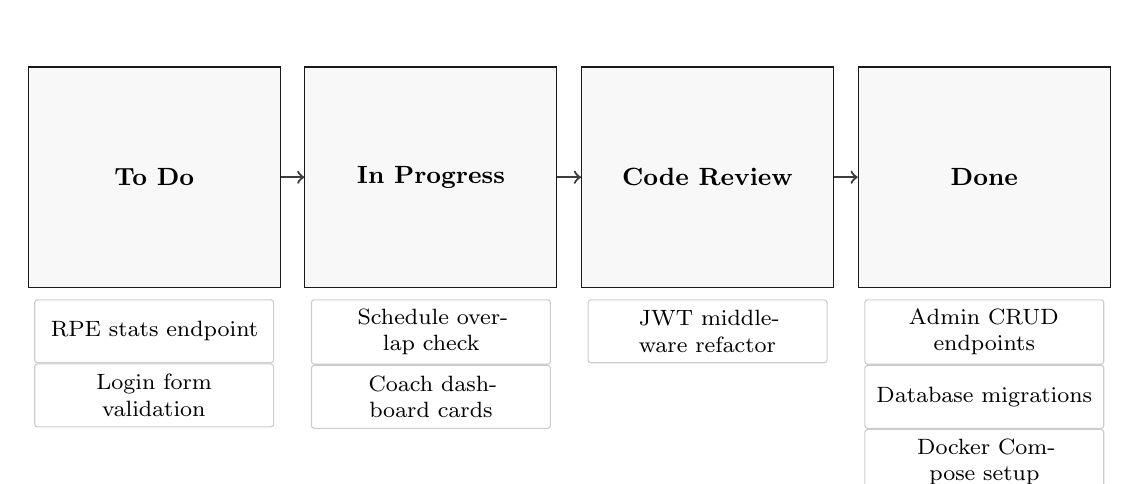
\begin{tikzpicture}[node distance=0.5cm, auto]
  \tikzstyle{stage} = [rectangle, draw=Black, fill=OffWhite, minimum width=3.2cm, minimum height=2.8cm, text centered, font=\small]
  \tikzstyle{task} = [rectangle, draw=BorderGray, fill=White, text width=2.8cm, minimum height=0.8cm, text centered, font=\footnotesize, rounded corners=1pt]
  
  \node [stage] (todo) {\textbf{To Do}};
  \node [stage, right=0.3cm of todo] (progress) {\textbf{In Progress}};
  \node [stage, right=0.3cm of progress] (review) {\textbf{Code Review}};
  \node [stage, right=0.3cm of review] (done) {\textbf{Done}};
  
  \node [task, below=0.15cm of todo.center, yshift=-1.4cm] (t1) {RPE stats endpoint};
  \node [task, below=0cm of t1] (t2) {Login form validation};
  
  \node [task, below=0.15cm of progress.center, yshift=-1.4cm] (p1) {Schedule overlap check};
  \node [task, below=0cm of p1] (p2) {Coach dashboard cards};
  
  \node [task, below=0.15cm of review.center, yshift=-1.4cm] (r1) {JWT middleware refactor};
  
  \node [task, below=0.15cm of done.center, yshift=-1.4cm] (d1) {Admin CRUD endpoints};
  \node [task, below=0cm of d1] (d2) {Database migrations};
  \node [task, below=0cm of d2] (d3) {Docker Compose setup};
  
  \draw[->, thick, DarkGray] (todo.east) -- (progress.west);
  \draw[->, thick, DarkGray] (progress.east) -- (review.west);
  \draw[->, thick, DarkGray] (review.east) -- (done.west);
\end{tikzpicture}
\end{center}

\vspace{6pt}
This kept us honest. At any point, anyone could check Jira and see exactly where things stood. Slack made sure nobody missed a notification — especially when a build broke at 11pm.

\newpage

%% ═════════════════════════════════════════════════════════════════════════════
\section{Rules of the System}
%% ═════════════════════════════════════════════════════════════════════════════

These are the constraints we baked into the code — not just "nice to have," but enforced at the database and API level.

\begin{tabularx}{\linewidth}{C{0.8cm} X L{4cm}}
\toprule
\hrow \# & Rule & How it's enforced \\
\midrule
1 & A boxer belongs to exactly one coach — period. & Foreign key \texttt{coach\_id} NOT NULL on the boxers table. No sharing. \\
\altrow 2 & Two sessions can't overlap in the same schedule. & Backend checks \texttt{start\_time} and \texttt{end\_time} before saving. \\
3 & Only coaches can record RPE. Boxers can't self-report. & The POST /rpe endpoint checks the JWT token role — rejects non-coaches. \\
\altrow 4 & Admin creates coaches manually. No public signup. & POST /coaches is behind admin authentication. \\
5 & Schedules are organized by month (YYYY-MM format). & Schedule schema enforces this — no free-form dates. \\
\altrow 6 & Analytics are computed on request, not cached. & Every analytics endpoint queries the DB fresh. We'll add Redis in v2 if needed. \\
\bottomrule
\end{tabularx}

\subsection{Performance targets (what we're aiming for)}

\begin{itemize}
  \item \textbf{v1 (Algeria pilot):} 40 coaches, $\sim$10 req/min peak, Render free tier.
  \item \textbf{Production:} 1,000 coaches, 60 req/min, p95 response time under 300ms.
  \item \textbf{Uptime:} 99.5\% on VPS. Render free tier is "best effort" (we know it can sleep).
\end{itemize}

\newpage

%% ═════════════════════════════════════════════════════════════════════════════
\section{The Data — Tables and Relationships}
%% ═════════════════════════════════════════════════════════════════════════════

Seven tables. Nothing complicated — just enough to model the domain.

\begin{tabularx}{\linewidth}{C{0.5cm} L{2.5cm} L{2cm} X}
\toprule
\hrow \# & Table & Module & What it stores \\
\midrule
01 & \texttt{admins} & Auth & Admin accounts — email, hashed password \\
\altrow 02 & \texttt{coaches} & Coaches & Coach profiles — created by an admin \\
03 & \texttt{boxers} & Boxers & Athlete data — linked to one coach \\
\altrow 04 & \texttt{schedules} & Planning & Monthly training schedules \\
05 & \texttt{sessions} & Planning & Individual sessions within a schedule \\
\altrow 06 & \texttt{exercises} & Planning & Exercises within a session \\
07 & \texttt{rpe\_entries} & RPE & Effort/fatigue records per boxer per session \\
\bottomrule
\end{tabularx}

\vspace{8pt}
\begin{calloutbox}
\textbf{How they connect:} 
Admin $\rightarrow$ creates Coach $\rightarrow$ Coach owns Boxers, Schedules.
Schedule $\rightarrow$ contains Sessions $\rightarrow$ Session $\rightarrow$ contains Exercises.
Boxer $\rightarrow$ has RPE Entries (optionally linked to a Session).
\end{calloutbox}

\subsection{admins}

Simple auth table. UUID primary key, email as unique login, bcrypt-hashed password.

\subsection{coaches}

\begin{tabularx}{\linewidth}{L{2.5cm} L{2.5cm} L{2cm} X}
\toprule
\hrow Column & Type & Constraint & Notes \\
\midrule
id & UUID & PK & \\
\altrow email & TEXT & UNIQUE & Login \\
password & TEXT & — & Hashed \\
\altrow full\_name & TEXT & — & \\
status & ENUM & — & active / inactive \\
\altrow created\_by & UUID & FK $\rightarrow$ admins & Who created this coach \\
created\_at & TIMESTAMPTZ & — & \\
\bottomrule
\end{tabularx}

\subsection{boxers}

This is where the athlete data lives. We added height and weight as optional fields — useful for weight class management.

\begin{tabularx}{\linewidth}{L{2.5cm} L{2.5cm} L{2cm} X}
\toprule
\hrow Column & Type & Constraint & Notes \\
\midrule
id & UUID & PK & \\
\altrow coach\_id & UUID & FK $\rightarrow$ coaches · NOT NULL & Exclusive ownership \\
first\_name & TEXT & — & \\
\altrow last\_name & TEXT & — & \\
email & TEXT & — & Optional — for future login \\
\altrow height & INT & — & cm (optional) \\
weight & FLOAT & — & kg (optional) \\
\altrow age & INT & — & \\
picture & TEXT & — & URL (optional) \\
\bottomrule
\end{tabularx}

\subsection{schedules}

Schedules are organized by month. The \texttt{month} field uses YYYY-MM format (e.g., "2026-03"). This makes filtering and navigation straightforward.

\subsection{sessions}

Each session belongs to a schedule, has a date, start time, and end time. The overlap check happens here before insert.

\subsection{exercises}

Exercises live inside sessions. For now, just a name and optional description. We kept it minimal — coaches can type whatever they need.

\subsection{rpe\_entries}

This is the core of the performance tracking system. We record:
\begin{itemize}
  \item \texttt{session\_rpe} (1–10 Borg CR-10 scale) — how hard the session felt
  \item \texttt{fatigue}, \texttt{sleep\_quality}, \texttt{soreness}, \texttt{stress} — optional 1–10 scales
  \item \texttt{entry\_date} — when the entry was recorded
  \item Linked to both \texttt{boxer\_id} (mandatory) and \texttt{session\_id} (optional — RPE can be recorded outside a formal session)
\end{itemize}

\newpage

%% ═════════════════════════════════════════════════════════════════════════════
\section{API Reference}
%% ═════════════════════════════════════════════════════════════════════════════

All endpoints live under \texttt{/api/}. Authentication is via \texttt{Authorization: Bearer <token>} header. Each endpoint checks the token and rejects requests from wrong roles.

\subsection{Auth — \texttt{/api/auth}}

\begin{tabularx}{\linewidth}{L{1.2cm} L{5cm} L{1.5cm} X}
\toprule
\hrow Method & Endpoint & Auth & What it does \\
\midrule
\methodpost & \texttt{/auth/admin/login} & No & Admin login — returns JWT \\
\altrow \methodpost & \texttt{/auth/coach/login} & No & Coach login — returns JWT \\
\methodpost & \texttt{/auth/boxer/login} & No & Boxer login (future) \\
\altrow \methodget & \texttt{/auth/me} & Yes & Returns current user's profile + role \\
\bottomrule
\end{tabularx}

\subsection{Admins — \texttt{/api/admins}}

\begin{tabularx}{\linewidth}{L{1.2cm} L{5cm} L{1.5cm} X}
\toprule
\hrow Method & Endpoint & Auth & What it does \\
\midrule
\methodget & \texttt{/admins} & \roleadmin & List all admins \\
\altrow \methodpost & \texttt{/admins} & \roleadmin & Create an admin \\
\methodget & \texttt{/admins/\{id\}} & \roleadmin & Admin details \\
\altrow \methodput & \texttt{/admins/\{id\}} & \roleadmin & Update admin \\
\methoddelete & \texttt{/admins/\{id\}} & \roleadmin & Delete admin \\
\bottomrule
\end{tabularx}

\subsection{Coaches — \texttt{/api/coaches}}

\begin{tabularx}{\linewidth}{L{1.2cm} L{5cm} L{1.5cm} X}
\toprule
\hrow Method & Endpoint & Auth & What it does \\
\midrule
\methodget & \texttt{/coaches} & \roleadmin & List all coaches \\
\altrow \methodpost & \texttt{/coaches} & \roleadmin & Create coach (admin only) \\
\methodget & \texttt{/coaches/\{id\}} & \roleadmin & Coach profile + stats \\
\altrow \methodput & \texttt{/coaches/\{id\}} & \roleadmin & Update coach \\
\methoddelete & \texttt{/coaches/\{id\}} & \roleadmin & Deactivate/delete coach \\
\bottomrule
\end{tabularx}

\subsection{Boxers — \texttt{/api/boxers}}

\begin{tabularx}{\linewidth}{L{1.2cm} L{5cm} L{1.5cm} X}
\toprule
\hrow Method & Endpoint & Auth & What it does \\
\midrule
\methodget & \texttt{/boxers} & \rolecoach & Coach's own boxers \\
\altrow \methodpost & \texttt{/boxers} & \rolecoach & Add boxer (auto-linked to coach) \\
\methodget & \texttt{/boxers/\{id\}} & \rolecoach & Boxer detail + RPE history \\
\altrow \methodput & \texttt{/boxers/\{id\}} & \rolecoach & Update boxer \\
\methoddelete & \texttt{/boxers/\{id\}} & \rolecoach & Remove boxer \\
\bottomrule
\end{tabularx}

\subsection{Schedules — \texttt{/api/schedules}}

\begin{tabularx}{\linewidth}{L{1.2cm} L{5cm} L{1.5cm} X}
\toprule
\hrow Method & Endpoint & Auth & What it does \\
\midrule
\methodget & \texttt{/schedules} & \rolecoach & List schedules (filter by month) \\
\altrow \methodpost & \texttt{/schedules} & \rolecoach & Create schedule \\
\methodget & \texttt{/schedules/\{id\}} & \rolecoach & Schedule + sessions \\
\altrow \methodput & \texttt{/schedules/\{id\}} & \rolecoach & Update schedule \\
\methoddelete & \texttt{/schedules/\{id\}} & \rolecoach & Delete schedule \\
\bottomrule
\end{tabularx}

\subsection{Sessions — \texttt{/api/schedules/\{id\}/sessions}}

Sessions are nested under schedules. This makes the URL structure reflect the data model.

\begin{tabularx}{\linewidth}{L{1.2cm} L{5.5cm} L{1.5cm} X}
\toprule
\hrow Method & Endpoint & Auth & What it does \\
\midrule
\methodget & \texttt{/schedules/\{id\}/sessions} & \rolecoach & Sessions in a schedule \\
\altrow \methodpost & \texttt{/schedules/\{id\}/sessions} & \rolecoach & Add session (overlap checked) \\
\methodget & \texttt{/schedules/sessions/\{id\}} & \rolecoach & Session detail + exercises \\
\altrow \methodput & \texttt{/schedules/sessions/\{id\}} & \rolecoach & Update session \\
\methoddelete & \texttt{/schedules/sessions/\{id\}} & \rolecoach & Delete session \\
\bottomrule
\end{tabularx}

\subsection{Exercises — \texttt{/api/sessions/\{id\}/exercises}}

Exercises are nested under sessions.

\begin{tabularx}{\linewidth}{L{1.2cm} L{5.5cm} L{1.5cm} X}
\toprule
\hrow Method & Endpoint & Auth & What it does \\
\midrule
\methodget & \texttt{/sessions/\{id\}/exercises} & \rolecoach & Exercises in a session \\
\altrow \methodpost & \texttt{/sessions/\{id\}/exercises} & \rolecoach & Add exercise \\
\methodput & \texttt{/sessions/exercises/\{id\}} & \rolecoach & Update exercise \\
\altrow \methoddelete & \texttt{/sessions/exercises/\{id\}} & \rolecoach & Delete exercise \\
\bottomrule
\end{tabularx}

\subsection{RPE — \texttt{/api/rpe}}

\begin{tabularx}{\linewidth}{L{1.2cm} L{5cm} L{1.5cm} X}
\toprule
\hrow Method & Endpoint & Auth & What it does \\
\midrule
\methodpost & \texttt{/rpe} & \rolecoach & Record RPE entry \\
\altrow \methodget & \texttt{/rpe/entries} & \rolecoach & All entries (filterable) \\
\methodget & \texttt{/rpe/boxer/\{id\}} & \rolecoach & Boxer's RPE history \\
\altrow \methodget & \texttt{/rpe/entry/\{id\}} & \rolecoach & Single entry \\
\methodput & \texttt{/rpe/entry/\{id\}} & \rolecoach & Update entry \\
\altrow \methoddelete & \texttt{/rpe/entry/\{id\}} & \rolecoach & Delete entry \\
\methodget & \texttt{/rpe/stats/\{id\}} & \rolecoach & Aggregated stats for boxer \\
\bottomrule
\end{tabularx}

\subsection{Analytics — \texttt{/api/analytics}}

\begin{tabularx}{\linewidth}{L{1.2cm} L{5.5cm} L{1.5cm} X}
\toprule
\hrow Method & Endpoint & Auth & What it does \\
\midrule
\methodget & \texttt{/analytics/admin/dashboard} & \roleadmin & Global stats overview \\
\altrow \methodget & \texttt{/analytics/admin/coach-athletes} & \roleadmin & Coach-athlete mapping \\
\methodget & \texttt{/analytics/admin/coaches-year} & \roleadmin & Yearly breakdown \\
\altrow \methodget & \texttt{/analytics/admin/boxers} & \roleadmin & Boxer-level analytics \\
\methodget & \texttt{/analytics/coach/dashboard} & \rolecoach & Coach's own dashboard \\
\altrow \methodget & \texttt{/analytics/coach/today-sessions} & \rolecoach & Today's sessions \\
\methodget & \texttt{/analytics/coach/ongoing-session} & \rolecoach & Currently running sessions \\
\bottomrule
\end{tabularx}

\newpage

%% ═════════════════════════════════════════════════════════════════════════════
\section{Frontend — What the User Sees}
%% ═════════════════════════════════════════════════════════════════════════════

\subsection{Page structure}

The frontend is a React SPA. No server-side rendering — just a clean client-side app that talks to the API. We built separate dashboards for admin and coach, since they have completely different needs.

\begin{itemize}
  \item \textbf{Landing page} — public. Explains what Zephyr is, links to login.
  \item \textbf{Admin dashboard} — Home (analytics overview), Manage Coaches (table + create/edit modals), Manage Admins, Settings/Profile.
  \item \textbf{Coach dashboard} — Home (own analytics, today's sessions), Manage Athletes (boxer list, profiles, RPE history), Schedules (monthly calendar, session builder), RPE (entry form, history view), Settings/Profile.
  \item \textbf{Boxer dashboard} — planned for later. Boxers will eventually log in to see their own progress charts.
\end{itemize}

\subsection{Responsive design}

We focused on desktop and tablet. Most coaches will use this on a laptop or tablet during training — not on a phone while coaching.

\begin{itemize}
  \item Desktop ($\geq$ 1280px) — full layout with sidebar and rich data tables.
  \item Tablet (768px – 1279px) — collapsible sidebar, stacked layouts where needed.
  \item Mobile — not a priority for v1, but the foundation is there if we need it.
\end{itemize}

\newpage

%% ═════════════════════════════════════════════════════════════════════════════
\section{Timeline — How We Built It}
%% ═════════════════════════════════════════════════════════════════════════════

We started development on March 9, 2026. Here's how the weeks played out.

\subsection{The plan, week by week}

\begin{adjustbox}{width=\linewidth, center}
\begin{ganttchart}[
    hgrid,
    vgrid={*1{draw=BorderGray, line width=0.1pt}},
    canvas/.style={fill=White},
    title/.style={fill=Black, draw=Black, text=White, font=\small},
    bar/.style={fill=RedMain, draw=RedDark},
    incomplete/.style={fill=LightGray, draw=BorderGray},
    bar height=0.45,
    y unit title=0.5cm,
    y unit chart=0.65cm,
    x unit=0.2cm,
    time slot format=isodate
]{2026-03-09}{2026-05-03}
    
    \gantttitlecalendar{year, month=shortname, week=1} \\
    
    \ganttgroup{Backend Development}{2026-03-09}{2026-03-22} \\
    \ganttbar[bar/.style={fill=RedMain, draw=RedDark}]{API + Database}{2026-03-09}{2026-03-22} \\
    \ganttbar[bar/.style={fill=MidGray, draw=DarkGray}]{Design (parallel)}{2026-03-09}{2026-03-22} \\
    
    \ganttgroup{Backend Deploy}{2026-03-23}{2026-03-24} \\
    \ganttbar{Render setup}{2026-03-23}{2026-03-24} \\
    
    \ganttgroup{Admin Dashboard}{2026-03-25}{2026-04-07} \\
    \ganttbar{React admin UI}{2026-03-25}{2026-04-07} \\
    
    \ganttgroup{Frontend Deploy}{2026-04-08}{2026-04-09} \\
    \ganttbar{First deploy}{2026-04-08}{2026-04-09} \\
    
    \ganttgroup{Coach Dashboard}{2026-04-10}{2026-04-23} \\
    \ganttbar{React coach UI}{2026-04-10}{2026-04-23} \\
    
    \ganttgroup{QA \& Production}{2026-04-24}{2026-05-01} \\
    \ganttbar{Final testing}{2026-04-24}{2026-05-01}
    
\end{ganttchart}
\end{adjustbox}

\subsection{What happened at each milestone}

\begin{itemize}
  \item \textbf{March 9 — Kickoff:} Project started. Set up repos, Docker environment, initial DB schema.
  \item \textbf{March 22 — API Ready:} All endpoints implemented and tested. Swagger docs auto-generated. Backend deployed to Render.
  \item \textbf{April 7 — Admin Dashboard:} Admin can log in, manage coaches and other admins, see analytics.
  \item \textbf{April 23 — Coach Dashboard:} Coach can manage athletes, create schedules and sessions, record RPE.
  \item \textbf{May 1 — Production:} Migrated to Hetzner VPS. Real coaches onboarded in Algeria.
\end{itemize}

Total: about 9.5 weeks from start to production.

\newpage

%% ═════════════════════════════════════════════════════════════════════════════
\section{Deployment and Costs}
%% ═════════════════════════════════════════════════════════════════════════════

\subsection{Infrastructure}

We use Docker Compose to run three services:
\begin{itemize}
  \item \textbf{API} — Python 3.11, FastAPI, Uvicorn with 4 workers
  \item \textbf{Database} — PostgreSQL 15 on Alpine
  \item \textbf{Reverse proxy} — Nginx for routing, HTTPS via Let's Encrypt
\end{itemize}

\subsection{Hosting phases and costs}

\begin{tabularx}{\linewidth}{L{2.8cm} L{2.5cm} L{2.5cm} L{2cm} X}
\toprule
\hrow Phase & Where & Capacity & Cost/mo & Status \\
\midrule
Phase 1 & Render free & $\sim$10 req/min & 0 € & 40 coaches — Algeria pilot \\
\altrow Phase 2 & Hetzner CX21 & 60 req/min & $\sim$5.77 € & 100 coaches \\
Phase 3 & Hetzner CX31 & 150+ req/min & $\sim$13.90 € & 1,000 coaches \\
\bottomrule
\end{tabularx}

\subsection{What 1,000 coaches looks like on a VPS}

\begin{tabularx}{\linewidth}{L{3cm} L{3cm} L{3cm} X}
\toprule
\hrow Resource & CX21 (entry) & CX31 (recommended) & Notes \\
\midrule
CPU & 2 vCPU & 2 vCPU & FastAPI handles async well \\
\altrow RAM & 4 GB & 8 GB & 8 GB gives breathing room \\
Storage & 40 GB & 80 GB & More than enough for now \\
\altrow Bandwidth & 20 TB & 20 TB & Won't come close to this \\
Price & 5.77 € & 13.90 € & \textbf{CX31 is the safer choice} \\
\bottomrule
\end{tabularx}

\subsection{What we'll change when we scale}

\begin{itemize}
  \item \textbf{Load balancer + multiple API replicas} — if one Uvicorn instance isn't enough
  \item \textbf{PgBouncer} — connection pooling for PostgreSQL
  \item \textbf{Redis} — cache frequent analytics queries (don't recompute "top performers" every request)
  \item \textbf{S3/MinIO} — for storing boxer profile images rather than local disk
\end{itemize}

None of this is needed for v1. It's just the plan.

\newpage

%% ═════════════════════════════════════════════════════════════════════════════
\section{What's Next}
%% ═════════════════════════════════════════════════════════════════════════════

\subsection{Near term (Phase 2)}

\begin{itemize}
  \item \textbf{Better analytics for coaches} — progress charts per boxer (RPE trend over time, fatigue patterns). This is the most requested feature from our pilot coaches.
  \item \textbf{Expand in Algeria} — from 40 to 100 coaches. Validate the system under more load.
\end{itemize}

\subsection{Medium term (Phase 3)}

\begin{itemize}
  \item \textbf{Boxer self-service} — athletes get their own login and can see their RPE history, training schedule, and progress. Reduces the coach's burden of being the only information source.
  \item \textbf{Notifications} — remind boxers of upcoming sessions via email (or push, eventually).
  \item \textbf{Redis caching} — when analytics start getting slow under load.
\end{itemize}

\subsection{Long term (Phase 4+)}

\begin{itemize}
  \item \textbf{AI-powered suggestions} — based on RPE history, the system could suggest when a boxer needs more rest or when they're ready to push harder. We're looking at GPT-4o for generating coaching recommendations.
  \item \textbf{Mobile app} — React Native, for coaches who want to record RPE from the gym floor.
  \item \textbf{International expansion} — Maghreb region first (Morocco, Tunisia), then global.
\end{itemize}

\subsection{Geographic rollout plan}

\begin{tabularx}{\linewidth}{L{3.5cm} L{3.5cm} L{3cm} X}
\toprule
\hrow Stage & Market & Coaches & Infrastructure \\
\midrule
Pilot & Algeria & 40 & Render free \\
\altrow Expansion & Algeria & 100 & Hetzner CX21 \\
Regional & Maghreb & 300+ & Hetzner CX31 \\
\altrow Global & International & 1,000+ & Multi-VPS or cloud \\
\bottomrule
\end{tabularx}

\newpage

%% ═════════════════════════════════════════════════════════════════════════════
\section{Security}
%% ═════════════════════════════════════════════════════════════════════════════

We take security seriously. Here's the approach:

\begin{itemize}
  \item \textbf{JWT with short-lived tokens} — access tokens last 15–60 minutes. Refresh tokens last 7 days. If a token leaks, it's only valid for a short window.
  \item \textbf{Role-based access control} — every endpoint checks the token's role claim. A coach can't hit admin endpoints and vice versa.
  \item \textbf{Data isolation} — coaches can only access their own boxers and schedules. The \texttt{coach\_id} filter is applied at the query level, not just in the UI.
  \item \textbf{Passwords} — bcrypt with 12 rounds. No plaintext, ever.
  \item \textbf{HTTPS} — enforced via Nginx + Let's Encrypt. HSTS in production.
  \item \textbf{Rate limiting} — 60 req/min per IP via SlowAPI middleware. Basic protection against brute force and scrapers.
\end{itemize}

\subsection{Non-functional requirements}

\begin{tabularx}{\linewidth}{L{3cm} L{4cm} X}
\toprule
\hrow Category & Metric & Target \\
\midrule
Response time & p95 latency & < 300ms \\
\altrow Availability & Monthly uptime & 99.5\% \\
Test coverage & Endpoints covered & > 80\% \\
\altrow Docs & OpenAPI/Swagger & Auto-generated, always current \\
Languages (future) & i18n support & French + Arabic \\
\bottomrule
\end{tabularx}

\vspace{16pt}

\begin{notebox}
\textbf{A note on completeness}

This spec covers everything we've built and everything we plan to build. The data models, API endpoints, business rules, frontend structure, deployment plan, and roadmap are all here. No hand-waving — every section corresponds to actual code in the repo. If something changes, this document gets updated. Simple as that.
\end{notebox}

\vspace{12pt}
\begin{center}
\small\color{MidGray}
Zephyr Boxing Coach System \quad·\quad 2026 \quad·\quad Built in Algeria, for coaches everywhere
\end{center}

\end{document}